\documentclass[11pt,a4paper]{article}

% =====================================================================
% UiT-inspired preamble
% Writing Scientific Reports in Computer Science & Engineering
% =====================================================================

% ---------------------------------------------------------------------
% Language / fonts / encoding
% ---------------------------------------------------------------------
\usepackage[utf8]{inputenc}
\usepackage[T1]{fontenc}
\usepackage[english]{babel}

% expansion disabled because lmodern is not installed
\usepackage{xcolor}
\usepackage[expansion=false]{microtype}

% ---------------------------------------------------------------------
% Page geometry and spacing
% ---------------------------------------------------------------------
\usepackage[margin=2.5cm]{geometry}
\usepackage{setspace}
\onehalfspacing

% ---------------------------------------------------------------------
% UiT colour palette
% ---------------------------------------------------------------------

% Main colour - Mørk blå
\definecolor{uitDarkBlue}{RGB}{0,51,73}

% Blue
\definecolor{uitBlue}{RGB}{0,115,150}

% Light blue
\definecolor{uitLightBlue}{RGB}{89,190,201}

% Red
\definecolor{uitRed}{RGB}{203,51,59}

% Yellow
\definecolor{uitYellow}{RGB}{242,169,0}

% ---------------------------------------------------------------------
% Math, figures, tables
% ---------------------------------------------------------------------
\usepackage{amsmath,amssymb,amsthm}
\usepackage{graphicx}
\usepackage{booktabs}
\usepackage{caption}
\usepackage{subcaption}

% ---------------------------------------------------------------------
% TikZ / PGFPlots
% ---------------------------------------------------------------------
\usepackage{tikz}
\usepackage{pgfplots}
\pgfplotsset{compat=1.18}
\usepackage{eso-pic}

% ---------------------------------------------------------------------
% Algorithms and code listings
% ---------------------------------------------------------------------
\usepackage[ruled,vlined,linesnumbered]{algorithm2e}
\usepackage{listings}

% Code colours based on UiT palette
\definecolor{codebg}{RGB}{245,247,248}
\definecolor{codekw}{RGB}{0,51,73}
\definecolor{codecomment}{RGB}{60,110,110}
\definecolor{codestring}{RGB}{203,51,59}

\lstdefinestyle{cs}{
  backgroundcolor=\color{codebg},
  basicstyle=\ttfamily\small,
  keywordstyle=\color{codekw}\bfseries,
  commentstyle=\color{codecomment}\itshape,
  stringstyle=\color{codestring},
  numbers=left,
  numberstyle=\tiny\color{uitDarkBlue},
  numbersep=8pt,
  frame=single,
  rulecolor=\color{uitLightBlue},
  breaklines=true,
  showstringspaces=false,
  tabsize=2,
  captionpos=b
}

\lstset{style=cs}

% ---------------------------------------------------------------------
% References
% ---------------------------------------------------------------------
% natbib + BibTeX is used for broad compatibility with TeX Live,
% MiKTeX, and Overleaf. No biber binary is required.
\usepackage[numbers,sort&compress]{natbib}

% ---------------------------------------------------------------------
% Lists
% ---------------------------------------------------------------------
\usepackage{enumitem}

% ---------------------------------------------------------------------
% Hyperlinks
% ---------------------------------------------------------------------
\usepackage{hyperref}

\hypersetup{
  colorlinks=true,
  linkcolor=uitDarkBlue,
  citecolor=uitBlue,
  urlcolor=uitBlue,
  pdftitle={Writing Scientific Reports in Computer Science and Engineering},
  pdfauthor={Your Name}
}

% ---------------------------------------------------------------------
% Cross-referencing
% ---------------------------------------------------------------------
\usepackage[capitalise,noabbrev]{cleveref}

% ---------------------------------------------------------------------
% Headers and footers
% ---------------------------------------------------------------------
\usepackage{fancyhdr}

\pagestyle{fancy}
\setlength{\headheight}{30pt}

\fancyhf{}

% Left side of header
\fancyhead[L]{%
  \textcolor{uitDarkBlue}{%
    \textbf{Writing Scientific Reports in CS/Engineering}%
  }%
}

% Right side of header: UiT logo
\fancyhead[R]{%
  
\includegraphics[height=22pt]{images/UiT_logos/UiT_Logo_Eng_2l_Bla_RGB.png}%
}

% Page number in footer
\fancyfoot[C]{%
  \textcolor{uitDarkBlue}{\thepage}%
}

% UiT light-blue line below header
\renewcommand{\headrulewidth}{0.4pt}

\renewcommand{\headrule}{%
  {\color{uitLightBlue}%
   \hrule width\headwidth height\headrulewidth}%
}

% ---------------------------------------------------------------------
% UiT logo - title page background overlay
% ---------------------------------------------------------------------

\newcommand{\uitTitleLogo}{%
  \tikz[remember picture,overlay]{
    \node[
      anchor=north east,
      inner sep=0pt,
      xshift=-1.5cm,
      yshift=-1.2cm
    ] at (current page.north east) {%
      
\includegraphics[height=100pt]{images/UiT_logos/UiT_Segl_Eng_Bla_960px.png}%
    };
  }%
}

% ---------------------------------------------------------------------
% Teaching boxes
% ---------------------------------------------------------------------
\usepackage{tcolorbox}
\tcbuselibrary{skins,breakable}

% Tip
\newtcolorbox{tipbox}[1][]{
  colback=uitLightBlue!10,
  colframe=uitBlue,
  fonttitle=\bfseries\color{uitDarkBlue},
  title=Tip,
  breakable,
  #1
}

% Common pitfall
\newtcolorbox{pitfallbox}[1][]{
  colback=uitRed!7,
  colframe=uitRed,
  fonttitle=\bfseries\color{uitRed!7},
  title=Common pitfall,
  breakable,
  #1
}

% Exercise
\newtcolorbox{exercisebox}[1][]{
  colback=uitYellow!12,
  colframe=uitYellow!80!black,
  fonttitle=\bfseries\color{uitDarkBlue},
  title=Exercise,
  breakable,
  #1
}


\title{%
  \AddToHook{shipout/background}{%
  \ifnum\value{page}=1
    \uitTitleLogo
  \fi
}
  \Large
  \textcolor{uitDarkBlue}{%
    \textbf{Writing Scientific Reports in\\
    Computer Science and Engineering}%
  }
  \\[0.3em]
  \large
  A Practical Guide and \LaTeX{} Template for Bachelor Students
}

\author{
  Course: \emph{DTE-2602 Introduction to Machine Learning and Artifical Intelligence}\\
  Instructor: \emph{Roy Espen Olsen}
}

\date{\today}

\begin{document}

\maketitle

\begin{abstract}
This document has two purposes at once. First, it is a short course on how to
plan, structure, and write a scientific report in computer science(CS) and
engineering, aimed at bachelor students writing their first lab reports,
project reports, or thesis chapters. Second, the document \emph{is itself}
written in \LaTeX{} and is meant to be copied and reused as a starting
template: every section demonstrates the very techniques it describes ---
figures, tables, algorithms, code listings, equations, and citations are
all shown ``in the wild'' so that students can see the source and the
rendered result side by side. Read \cref{sec:structure} for the expected
structure of a report, and use \cref{sec:checklist} as a final
self-review checklist before submission.
\end{abstract}

\newpage
\tableofcontents
\thispagestyle{fancy}
\newpage

% Its not always necessary to add a \newline after each section, 
% but it is often done. It makes it easier to see where each new section starts.
\section{Introduction}
\label{sec:introduction}

A scientific report is not a diary entry, a sales pitch, or a code
comment expanded to ten pages. It is a structured argument: you had a
question or a problem, you did something about it in a principled way,
and you obtained results that a professor, teacher or even a stranger --- your reader --- can
understand, judge, and in principle reproduce. Everything in this guide
follows from that one sentence.

In computer science and engineering, this means your report typically
documents one of the following:
\begin{itemize}[nosep]
      \item an \textbf{experiment} (e.g.\ benchmarking two algorithms, evaluating
            a machine-learning model),
      \item a \textbf{system} you designed and built (e.g.\ a compiler, a web
            service, an embedded controller), or
      \item an \textbf{investigation} of an existing system or dataset.
\end{itemize}
In all three cases, the reader --- your instructor, a fellow student, or
your future self in six months --- should be able to answer three
questions after reading your report: \emph{What did you do? Why did you
do it that way? What did you find, and what does it mean?}

\begin{tipbox}
      Write for a reader who is intelligent and technically competent, but who
      was \emph{not} in the room when you did the work. They do not know what
      you meant to say --- only what you actually wrote.
\end{tipbox}

This document walks through the expected structure of a report
(\cref{sec:structure}), how to write clearly and in an appropriate
academic style (\cref{sec:style}), how to present figures, tables,
algorithms and code (\cref{sec:figures,sec:algorithms}), how to cite
sources correctly (\cref{sec:citations}), a few \LaTeX{}-specific tips
that will make your life easier (\cref{sec:latex-tips}), a list of
mistakes we see every year (\cref{sec:mistakes}), and a checklist to run
through before you submit (\cref{sec:checklist}).

\newpage
\section{Structure of a Report}
\label{sec:structure}

Most scientific writing in engineering follows a variant of the
\textbf{IMRaD} pattern: \emph{Introduction, Methods, Results, and
Discussion}. \Cref{tab:structure} shows how this maps onto a typical
CS/engineering report and what each part is \emph{for} --- not just what
it is called.

\renewcommand{\arraystretch}{1.4}

\begin{table}[htbp]
  \centering
  \caption{Typical section structure for a CS/engineering report and the
  question each section must answer.}
  \label{tab:structure}

  \begin{tabular}{@{}p{4cm}p{10.5cm}@{}}
    \toprule
    \textbf{Section} & \textbf{Question it must answer} \\
    \midrule

    Title & What is this, in one line? \\
    \hline
    Abstract & In 150--250 words: problem, approach, key result. \\
    \hline
    Introduction & Why does this problem matter, and what exactly did you do about it? \\
    \hline
    Background / Related Work & What does the reader need to know, and how does your work relate to existing solutions? \\
    \hline
    Design / Methodology & How does your system or experiment work, and why did you make these design choices? \\
    \hline
    Implementation & What did you actually build? (Only if relevant --- keep it high-level; code goes in an appendix or repository.) \\
    \hline
    Evaluation / Results & What did you measure, and what did you observe? (Facts only, no interpretation yet.) \\
    \hline
    Discussion & What do the results \emph{mean}? What are the limitations? \\
    \hline
    Conclusion & What is the one-paragraph takeaway, and what would you do next? \\
    \hline
    References & Who else's work did you build on or compare against? \\

    \bottomrule
  \end{tabular}
\end{table}

\subsection{Abstract}
The abstract is the most-read and least-understood part of a report. It
is \emph{not} an introduction and it is \emph{not} a table of contents in
prose form. A good abstract compresses the whole report into four moves:
(1) one sentence of context/problem, (2) one sentence of what you did,
(3) one or two sentences of what you found, (4) optionally, one sentence
on why it matters. Write the abstract \emph{last}, after the rest of the
report is stable.

\subsection{Introduction vs.\ Background}
Students often merge these, which weakens both. The \textbf{introduction}
motivates the problem and states your contribution in the first page ---
a reader who stops after the introduction should still know what you did
and why. The \textbf{background/related work} section is where you teach
the reader the prerequisites and position your work relative to existing
approaches. If a fact is needed to understand your method, it belongs in
background, not scattered later.

\begin{tipbox}
  A useful test: could you swap the introduction of two unrelated reports
  and have both still make sense? If yes, your introduction is too generic
  --- it needs to say what \emph{your} project specifically does.
\end{tipbox}

\subsection{Results vs.\ Discussion}
Keep these separate, even if only conceptually. \textbf{Results} report
what happened, ideally with a table or figure and minimal commentary.
\textbf{Discussion} is where you interpret: Was this expected? Does it
support your hypothesis? What are the threats to validity (measurement
noise, small sample, unrepresentative test data, hardware differences)?
Mixing the two makes it hard for a reader --- or a grader --- to tell
which sentences are evidence and which are your opinion.

\begin{exercisebox}
  Take the last report you wrote (for this course or another) and
  highlight every sentence in your results section that contains a
  judgement word (``surprisingly'', ``unfortunately'', ``clearly better'').
  Each one is arguably discussion, not results. How many did you find?
\end{exercisebox}

\newpage
\section{Writing Style}
\label{sec:style}
The primary goal of technical writing is to communicate ideas precisely
and efficiently. In a CS or engineering report, clear language is more
valuable than sophisticated-sounding language. The following guidelines
cover the main aspects of technical style: clarity, tense, voice, precision,
terminology, and paragraph structure.

\subsection{Clarity over cleverness}
Prefer the plain word to the fancy one, and the short sentence to the
long one. ``We used'' beats ``We made utilization of''. ``The algorithm
runs in $O(n\log n)$ time'' beats ``The algorithm exhibits logarithmic
scaling behaviour with respect to input cardinality''. If a sentence
takes two readings to parse, split it.

\subsection{Tense}
As a simple default:
\begin{itemize}[nosep]
      \item \textbf{Past tense} for what you did and what you observed:
            ``We evaluated three schedulers'', ``The cache hit rate dropped
            to 62\,\%''.
      \item \textbf{Present tense} for facts that remain true and for
            describing the content of your document itself: ``\Cref{fig:latency}
            shows the results'', ``TCP guarantees in-order delivery''.
\end{itemize}

\subsection{Passive vs.\ active voice, and first person}
Both active and passive voice are acceptable in engineering writing;
the goal is clarity, not a blanket rule. Active voice is usually more
direct: ``We measured latency under three loads'' is easier to parse than
``Latency was measured under three loads by us''. Passive voice is useful
when the actor is irrelevant or obvious: ``The packets were captured
using \texttt{tcpdump}'' is fine because \emph{who} ran the tool matters
less than \emph{how} the data was captured. Using ``we'' for actions your
team actually performed is standard in modern CS writing --- check your
course or venue's convention if unsure.

\begin{pitfallbox}
      Do not mix an impersonal, passive style in the results with a chatty
      ``I think'' style in the discussion. Pick a register and keep it
      consistent across the whole report.
\end{pitfallbox}

\subsection{Precision and hedging}
Say exactly what you mean and no more. ``The system is fast'' is not a
claim you can defend; ``the system processes 12{,}400 requests/s at the
95th-percentile latency of 8\,ms on the hardware described in the
experimental setup section'' is. Conversely, do not overclaim: if you tested on
one dataset, say so, and do not generalise to ``all workloads''. Words
like ``clearly'', ``obviously'', and ``trivially'' rarely help the
reader and often hide a step you skipped.

\subsection{Consistency}
Pick one term for each concept and stick to it. If your system is a
``scheduler'' in \cref{sec:structure}, do not call it a ``dispatcher'' in
the evaluation unless you have explicitly defined them as synonyms.
The same applies to notation: if $n$ is the number of nodes in
\cref{sec:algorithms}, it must still be the number of nodes on the last
page.

\subsection{Paragraph and section structure}
One idea per paragraph, and put the main point in the first sentence
(a ``topic sentence''). Readers --- and graders --- skim; a report whose
first sentence of every paragraph forms a coherent summary is a
well-structured report. Use subsections to help navigation, but avoid
sections with a single sentence and no subsections around them; if a
subsection is that short, it is probably a paragraph, not a subsection.

\begin{tipbox}
      Read your own paragraph's first sentence out loud, in order, skipping
      everything else. If that summary doesn't make sense as an outline of
      your argument, restructure the paragraphs.
\end{tipbox}

\newpage
\section{Figures and Tables}
\label{sec:figures}

Figures and tables carry evidence; captions carry meaning. A common
mistake is a one-line caption like ``Results'' under a plot with three
unlabelled axes. \Cref{fig:latency} shows a better pattern: the caption
states what is plotted, the axes, and the one-sentence takeaway, so the
figure is understandable even if a reader skips the surrounding text.

\begin{figure}[htbp]
  \centering
  \begin{tikzpicture}
    \begin{axis}[
        width=0.75\linewidth,
        height=5.5cm,
        xlabel={Concurrent clients},
        ylabel={p95 latency (ms)},
        xmin=0, xmax=110,
        ymin=0,
        grid=major,
        legend pos=north west,
        legend style={font=\small},
      ]
      \addplot[thick, mark=*, color=blue!70!black] coordinates {
        (1,4.1) (10,4.6) (20,5.3) (40,7.9) (60,12.4) (80,21.0) (100,38.5)
      };
      \addlegendentry{Baseline scheduler}
      \addplot[thick, mark=square*, color=orange!80!black] coordinates {
        (1,4.0) (10,4.3) (20,4.9) (40,6.1) (60,7.8) (80,10.2) (100,14.7)
      };
      \addlegendentry{Proposed scheduler}
    \end{axis}
  \end{tikzpicture}
  \caption{95th-percentile request latency versus number of concurrent
  clients, for the baseline round-robin scheduler and the proposed
  load-aware scheduler (\cref{sec:algorithms}). The proposed scheduler
  degrades more gracefully under load. \emph{(Illustrative numbers, not
  real measurements --- in your own report this caption should also
  point to the section describing your experimental setup.)}}
  \label{fig:latency}
\end{figure}

\begin{tipbox}
Every figure and table needs: a caption that stands on its own, labelled
axes with units, a legend if there is more than one series, and a
reference from the body text (``\texttt{\textbackslash cref\{fig:latency\}}
shows\ldots''). A figure the text never mentions is a figure the reader
will skip.
\end{tipbox}

\subsection{Tables}
Use tables for precise numbers the reader may want to look up; use
figures for trends and shapes. \Cref{tab:comparison} is a minimal
example using the \texttt{booktabs} package, which gives cleaner
horizontal rules than the default \LaTeX{} table style (avoid vertical
rules and ``double'' borders --- they add visual noise, not information).

\begin{table}[htbp]
  \centering
  \caption{Comparison of the two schedulers at 100 concurrent clients.
  Throughput in requests per second; latency in milliseconds.}
  \label{tab:comparison}
  \begin{tabular}{@{}lrrr@{}}
    \toprule
    Scheduler & Throughput (req/s) & p50 latency & p95 latency \\
    \midrule
    Baseline (round-robin) & 8{,}120  & 9.8 ms  & 38.5 ms \\
    Proposed (load-aware)  & 11{,}940 & 6.1 ms  & 14.7 ms \\
    \bottomrule
  \end{tabular}
\end{table}

\begin{pitfallbox}
  Do not screenshot a table from a spreadsheet or a terminal. Rebuild it
  natively in \LaTeX{} (as above) so that fonts, alignment, and decimal
  points match the rest of the document.
\end{pitfallbox}

\subsection{Placement and referencing}
Let \LaTeX{} place floats (\texttt{htbp}) rather than fighting it with
exact positions; refer to figures/tables by label
(\verb|\cref{fig:latency}|) rather than by position (``the figure
above''), since positions shift as the document is edited.

\newpage
\section{Algorithms and Code}
\label{sec:algorithms}
Algorithms and implementation details should be presented at the level
needed for the reader to understand, reproduce, or evaluate the work.
Use pseudocode when the logic of an algorithm is the important part, source
code listings when a specific implementation detail matters, and equations
when the underlying computation or relationship needs to be stated
precisely. Avoid reproducing implementation details that do not contribute
to the argument; the complete source code can instead be provided in an
appendix or repository.

\subsection{Pseudocode}
When the \emph{logic} of a method matters more than a specific programming
language, present it as pseudocode with the \texttt{algorithm2e} package,
as in \Cref{alg:kmeans}. Pseudocode should be language-agnostic, use
meaningful variable names, and be short enough to read in under a minute.
If it needs more than about 20 lines, summarise the outer loop in prose and
put the full version in an appendix.

\begin{algorithm}[htbp]
  \DontPrintSemicolon
  \KwIn{Dataset $X = \{x_1,\ldots,x_n\}$, number of clusters $k$}
  \KwOut{Cluster assignments $c_1,\ldots,c_n$ and centroids $\mu_1,\ldots,\mu_k$}

  Initialise $k$ centroids $\mu_1,\ldots,\mu_k$ randomly\;
  
  \Repeat{convergence}{
    \ForEach{$x_i \in X$}{
      $c_i \gets \arg\min_{j \in \{1,\ldots,k\}}
      \lVert x_i - \mu_j \rVert^2$\;
    }

    \ForEach{$j \in \{1,\ldots,k\}$}{
      $\mu_j \gets \frac{1}{|\{i : c_i=j\}|}
      \sum_{i:c_i=j} x_i$\;
    }
  }

  \Return{$c_1,\ldots,c_n,\mu_1,\ldots,\mu_k$}\;

  \caption{K-means clustering}
  \label{alg:kmeans}
\end{algorithm}

\subsection{Source code listings}
When the exact code matters (e.g.\ when explaining a preprocessing step or
a model implementation detail), use the \texttt{listings} package rather
than a screenshot, so the code is searchable, copy-pasteable, and
consistently styled. \Cref{lst:kmeans} shows a short Python implementation
using scikit-learn.

\begin{lstlisting}[language=Python,
  caption={Clustering data points with K-means.},
  label={lst:kmeans}]
from sklearn.cluster import KMeans

model = KMeans(n_clusters=3, random_state=42)
labels = model.fit_predict(X)
\end{lstlisting}

\begin{tipbox}
  Only include code that illustrates a specific point you are making in
  the text. A report is not the place to reproduce your entire codebase
  --- link to a repository or put long listings in an appendix.
\end{tipbox}

\begin{pitfallbox}
  Do not paste an indented code block as plain text without syntax
  highlighting or numbering; it becomes very hard to reference (``see line
  14'') and hard to read. Use \texttt{listings} or \texttt{minted}
  consistently throughout the report.
\end{pitfallbox}

\subsection{Equations}
Number equations you refer to later, and treat the equation as part of
the sentence grammatically. For example, the K-means objective can be
defined as

\begin{equation}
  \label{eq:kmeans}
  J =
  \sum_{i=1}^{n}
  \left\lVert x_i - \mu_{c_i} \right\rVert^2,
\end{equation}

where $x_i$ is the $i$th data point, $c_i$ is its assigned cluster, and
$\mu_{c_i}$ is the centroid of that cluster. \Cref{eq:kmeans} expresses
the objective that K-means minimises: the total squared distance between
each data point and the centroid of its assigned cluster. The equation
therefore gives the reader a precise mathematical description of the
algorithm presented in \Cref{alg:kmeans}.


\newpage
\section{Citations and References}
\label{sec:citations}
Citations make clear which ideas, methods, results, and resources come
from existing work and which are the author's own. They allow readers to
verify claims, locate the work on which the report builds, and distinguish
established knowledge from new contributions. This section explains when
citations are required, how to manage references with \LaTeX{}, and how to
cite software, datasets, and AI tools appropriately.

\subsection{Why and when to cite}
Cite a source whenever you rely on a fact, method, figure, or idea that
is not your own or not common knowledge in the field. This includes:
background facts (e.g.\ the original definition of an algorithm
\cite{dijkstra1959}), tools and datasets you used, and prior work you
compare against. A rule of thumb: if you could not have written the
sentence without having read that source, cite it. Foundational results
you build directly on should also be cited, even if they are famous ---
for example, referencing Shannon's original formulation when discussing
channel capacity \cite{shannon1948}.

\begin{pitfallbox}
  Citing a source is not the same as quoting it. Paraphrase in your own
  words and cite; use direct quotation marks only for the rare case where
  the exact wording matters (e.g.\ a definition from a standard).
  Copy-pasting text and adding a citation at the end of the paragraph is
  still plagiarism if the wording is not your own.
\end{pitfallbox}

\subsection{Using \texttt{natbib} and BibTeX}
This template uses \texttt{natbib} with the \texttt{ieeetr} bibliography
style, a numeric style common in CS/engineering venues. Entries live in
\texttt{references.bib}; a minimal entry looks like:

\begin{lstlisting}[language=TeX, caption={A BibTeX entry.}]
@inproceedings{smith2023scheduling,
  author    = {Smith, Jane and Doe, John},
  title     = {Load-Aware Scheduling for Microservices},
  booktitle = {Proc. of ExampleConf},
  year      = {2023},
  pages     = {1--12},
}
\end{lstlisting}

and is cited in the text with \verb|\cite{smith2023scheduling}|, which
renders as a bracketed number with the \texttt{ieeetr} style used here,
e.g.\ the classic paper on machine intelligence \cite{turing1950}. (If
you use an author--year style such as \texttt{plainnat} or
\texttt{biblatex}'s \texttt{authoryear} instead, \texttt{natbib}'s
\verb|\citet{...}| lets you use the author name as a noun in the
sentence, e.g.\ ``Turing \verb|\citet{turing1950}| asked whether
machines can think.'') Every entry you cite must appear in
\texttt{references.bib},
and (with numeric styles) every entry in the bibliography should be
cited somewhere --- do not pad the reference list.

\begin{tipbox}
  If your own \LaTeX{} install has \texttt{biblatex}/\texttt{biber}
  available (true on Overleaf and most modern TeX Live installs), you can
  swap this template's \texttt{natbib} block in \texttt{main.tex} for
  \verb|\usepackage[backend=biber,style=ieee]{biblatex}| plus
  \verb|\addbibresource{references.bib}| and
  \verb|\printbibliography|; \texttt{biblatex} offers more citation
  styles and better internationalisation. Both approaches read the same
  \texttt{references.bib} file.
\end{tipbox}

\subsection{Citing software, datasets, and AI tools}
Cite the tools and datasets that materially shaped your results, e.g.\ a
specific library version, dataset, or pretrained model, the same way you
would cite a paper --- most have a recommended citation in their
documentation or a Zenodo/DOI record. If you used a generative AI tool
(e.g.\ for code suggestions or editing), follow your course's or
institution's disclosure policy; when in doubt, state in a short
paragraph (e.g.\ at the end of the introduction or in an
acknowledgements section) what the tool was used for and confirm you
verified the result yourself.

\begin{tipbox}
  Keep an eye on citation style consistency: IEEE numeric
  (\texttt{[1]}), ACM, or author--year (APA/Chicago) --- pick the one your
  course requires and use it throughout. Reference managers (Zotero,
  JabRef) export directly to \texttt{.bib} and will save you many hours
  over a semester.
\end{tipbox}

\newpage
\section{Practical \LaTeX{} Tips}
\label{sec:latex-tips}

This section is about the tool, not the writing --- small habits that
save time and prevent embarrassing errors.

\begin{itemize}
      \item \textbf{One file per section.} As in this project
            (\texttt{sections/*.tex}, pulled in with \verb|\input{}|), split
            long documents so you can navigate, diff, and collaborate more
            easily via version control.
      \item \textbf{Use \texttt{cleveref}.} Write \verb|\cref{fig:latency}|
            instead of \verb|Figure~\ref{fig:latency}|; it automatically
            inserts ``Figure'', ``Table'', ``Section'', etc., consistently,
            and you only need to remember one command.
      \item \textbf{Never hand-number figures/sections/equations.} Always use
            \verb|\label{}| and \verb|\ref{}|/\verb|\cref{}|. Manually typed
            numbers (``see Figure 3'') silently go stale the moment you add a
            figure earlier in the document.
      \item \textbf{Non-breaking spaces before references.} Write
            \verb|Section~\ref{sec:x}| (with \verb|~|) --- \texttt{cleveref}
            handles this automatically, which is one more reason to use it.
      \item \textbf{Use version control.} Put the project in Git. \LaTeX{}
            source is plain text and diffs beautifully; commit before major
            rewrites so you can always go back.
      \item \textbf{Compile often.} Do not write for an hour without
            compiling --- errors are much easier to find one paragraph at a
            time than after 300 new lines.
      \item \textbf{\texttt{siunitx} for units and numbers.} For a
            report with many measurements, the \texttt{siunitx} package
            (e.g.\ \verb|\SI{8.2}{ms}|) keeps units and number formatting
            consistent; not used in this template to keep dependencies
            minimal, but worth adding for data-heavy reports.
      \item \textbf{Spell- and grammar-check.} Use your editor's checker or
            an external tool before submission; typos undermine an otherwise
            good report.
      \item \textbf{Keep the preamble organised.} As the document grows, move
      packages and custom commands into a separate \texttt{preamble.tex}
      file and load it from \texttt{main.tex} with \verb|\input|. This keeps
      the main document focused on its content and makes the configuration
      easier to maintain.
\end{itemize}

\begin{tipbox}
      Compile with \texttt{latexmk -pdf main.tex} (or the provided
      \texttt{Makefile}: run \texttt{make}) rather than calling
      \texttt{pdflatex} manually several times --- \texttt{latexmk} re-runs
      \texttt{bibtex}/\texttt{pdflatex} exactly as many times as needed to
      resolve citations and cross-references.
\end{tipbox}

\newpage
\section{Common Mistakes We See Every Year}
\label{sec:mistakes}

The following are common issues that weaken otherwise solid reports;
check for them before finalising your document.

\begin{enumerate}[nosep]
      \item \textbf{Abstract that only restates the title.} ``This report
            describes our load balancer'' tells the reader nothing an
            abstract should: what was the problem, what did you build, what
            did you find?
      \item \textbf{No explicit research question or goal.} If a reader
            cannot point to one sentence in your introduction that says what
            you set out to answer or build, the rest of the report has
            nothing to be evaluated against.
      \item \textbf{Results without a baseline or comparison.} ``Our system
            achieves 95\,\% accuracy'' means little without stating what a
            naive baseline achieves, or what prior work reports.
      \item \textbf{Screenshots instead of native figures/tables.} Hard to
            read, inconsistent fonts, and impossible to cross-reference
            cleanly (see \cref{sec:figures}).
      \item \textbf{Unlabelled axes or missing units.} A plot with axes
            called ``x'' and ``y'' communicates nothing.
      \item \textbf{Wall-of-code appendices with no explanation.} Code should
            support the argument, not replace it; explain the interesting 10
            lines rather than pasting 500.
      \item \textbf{Inconsistent notation or terminology}, e.g.\ switching
            between $n$ and $N$ for the same quantity, or between ``node''
            and ``server'' for the same concept.
      \item \textbf{Claims with no evidence}, e.g.\ ``this is clearly the
            best approach'' without a measurement, citation, or argument to
            support it.
      \item \textbf{Missing or informal citations}, e.g.\ ``according to a
            blog post I found'' instead of a proper reference, or reusing
            text from a source without paraphrasing and citing it
            (\cref{sec:citations}).
      \item \textbf{Conclusion that introduces new material.} The conclusion
            should summarise and reflect on what came before, not present
            new results or arguments for the first time.
      \item \textbf{Ignoring \LaTeX{} warnings.} ``Overfull \textbackslash
            hbox'', undefined references, and missing citations shown as
            ``\texttt{[?]}'' in the compiled PDF are not cosmetic --- fix them
            before submitting.
\end{enumerate}

\begin{pitfallbox}
      The single most common issue is not grammar --- it is \emph{structure}:
      results and discussion mixed together, no clear research question, or a
      conclusion that repeats the abstract word for word. Fix structure first;
      polish sentences last.
\end{pitfallbox}

\newpage
\section{Pre-submission Checklist}
\label{sec:checklist}

Run through this list before you submit. Most items take under a minute
and catch the mistakes graders notice first.

\subsection*{Content}
\begin{itemize}[nosep]
      \item[$\square$] The abstract states problem, approach, and key
            result in a few sentences.
      \item[$\square$] The introduction states the goal/research question
            explicitly and says what was done, in the first page.
      \item[$\square$] No heading is left without text introducing the
      following subsection.     
      \item[$\square$] Every figure and table has a caption that stands
            alone, labelled axes/units, and is referenced from the body
            text.
      \item[$\square$] Results are reported before they are interpreted;
            discussion is clearly separated from results.
      \item[$\square$] Claims are backed by a measurement, a citation, or an
            explicit argument --- not just asserted.
      \item[$\square$] Limitations/threats to validity are mentioned
            honestly.
      \item[$\square$] The conclusion summarises rather than introduces new
            material.
\end{itemize}

\subsection*{References}
\begin{itemize}[nosep]
      \item[$\square$] Every non-trivial claim taken from elsewhere is
            cited.
      \item[$\square$] Every entry in \texttt{references.bib} that is
            cited actually compiles (no ``\texttt{[?]}'' in the PDF).
      \item[$\square$] Citation style is consistent throughout.
\end{itemize}

\subsection*{Mechanics}
\begin{itemize}[nosep]
      \item[$\square$] The document compiles cleanly: no undefined
            references, no missing citations, no overfull boxes you have not
            checked.
      \item[$\square$] Notation and terminology are consistent from start to
            end.
      \item[$\square$] Spelling and grammar have been checked.
      \item[$\square$] Page/word limits (if any) are respected.
      \item[$\square$] Filenames and any submission instructions from the
            course have been followed.
\end{itemize}

\begin{tipbox}
      Read the report once, start to finish, out loud or to a friend, the
      evening before it is due (not the minute before). You will catch things
      a silent read misses.
\end{tipbox}

\newpage

\addcontentsline{toc}{section}{References}
\bibliographystyle{ieeetr}
\bibliography{references}

\end{document}
